\documentclass{beamer}
\mode<presentation>
\usepackage{tikz}
\usetikzlibrary{shapes.geometric,positioning,math}
\title{Playing with Pascal's Triangle}
\author[dishajk]{Disha Kuzhively}
\institute{ICTS-TIFR}
\date[VITM]{1 June 2025}
\begin{document}
\begin{frame}
    \titlepage
\end{frame}
\begin{frame}
    \frametitle{Outline}
    \tableofcontents[pausesections]
    \end{frame}
\section{Warm-up}
\begin{frame}
    \frametitle{Number of chocolates}
    \begin{block}{Problem}
        Maya brought home chocolates for her 6 children Asha, Bindu, Chaitra, Divya, Esha, and Farah. She gave them to the youngest, Farah and asked her to distribute them among her siblings. Farah ate half of the chocolates and gave the rest to Esha and asked her to distribute them among her younger siblings. Esha did the same, ate half and gave the rest to Divya and so on. In the end, the oldest child Asha got only one chocolate. How many chocolates did Maya bring home?
    \end{block}

    \uncover<2->{What if Maya had \alert{7} children instead of 6, what would be the number of chocolates Maya would have brought home then?}
\end{frame}
\begin{frame}
\frametitle{Sum of Numbers}
\begin{block}{Problem}
    Find the sum of \(1+2+4+8+\ldots+1024\).
\end{block}
\end{frame}
\begin{frame}
    \frametitle{Number of Routes}
    Below is the map of the city showing Maya's house and VITM. Maya visits VITM taking the shortest possible route.
    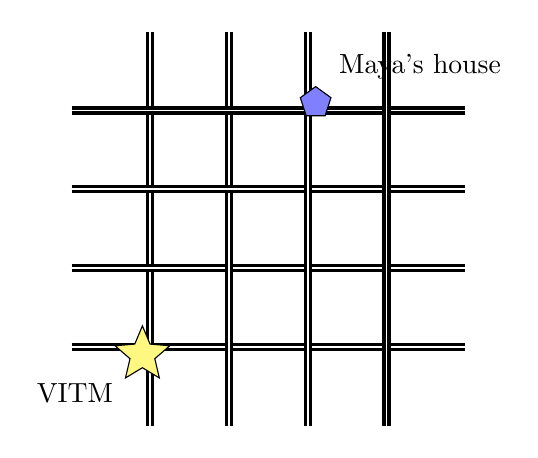
\begin{tikzpicture}
        \foreach \k in {0,1,...,3} {
          \draw[very thick, double] (0,\k) -- (5,\k);
          \draw[very thick, double] ({\k+1},-1) -- ({\k+1},4);
        }
        \node[star,star points=5,star point height=2mm,fill=yellow!50,draw] (m) at (0.9,-0.1) {};
        \node[below left=2pt of m] {VITM};
        \node[regular polygon,regular polygon sides=5,minimum size=2mm,fill=blue!50,draw] (n) at (3.1,3.1) {};
        \node[above right=2pt of n] {Maya's house};
      \end{tikzpicture}

    Maya visits VITM taking the shortest possible route.
  
    How many such routes are there?
\end{frame}
\begin{frame}
\frametitle{Highest number of routes}
The houses of 6 students who came to VITM today are marked in pentagons. 

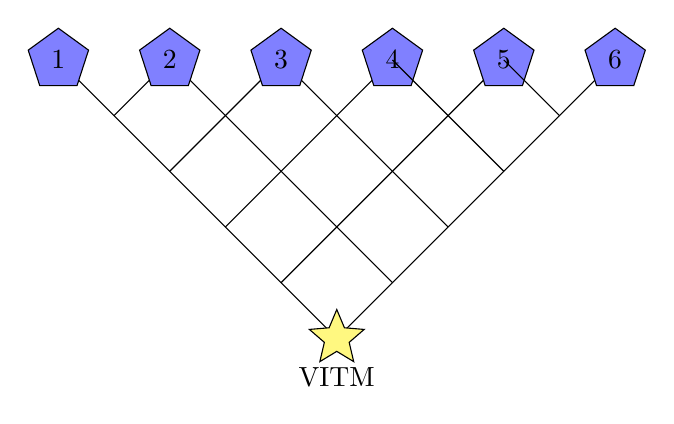
\begin{tikzpicture}
    \foreach \k in {0,1,...,5} {
        \pgfmathsetmacro{\h}{int(6 - \k)}
        \draw (135:\k)--++(45:{5-\k}) node[regular polygon,regular polygon sides=5,minimum size=2mm,fill=blue!50,draw] {\h};
        \draw (45:\k) --++ (135:{5-\k});
        }
    \node[star,star points=5,star point height=2mm,fill=yellow!50,draw] (m) at (0,0) {};
    \node[below=2pt of m] {VITM};
  \end{tikzpicture}

Which of these students have the highest number of routes to return home?

Keep in mind these students try to take the shortest possible routes. 
\end{frame}
\begin{frame}
\frametitle{Number of routes}
Write in every circle the number of ways that lead to it from the entrance.

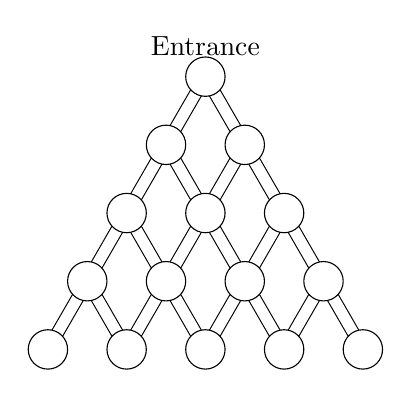
\begin{tikzpicture}[scale=1]
    \node[above=4pt] at (0,0) {Entrance};
    \pgfmathsetmacro{\r}{4}
    \foreach \y in {0,...,\r}{
        \draw[double distance=4pt] (-60:\y) --++ (-120:{\r-\y});
        \draw[double distance=4pt] (-120:\y) --++ (-60:{\r-\y});
        \foreach \x in {0,...,\y}{
        \draw[fill=white] ({\y/2-\x},{-\y*sqrt(3)/2}) circle (0.25);
      }
    }    
  \end{tikzpicture}
\end{frame}
\section{Pascal's Triangle}
\begin{frame}
    \frametitle{Pascal's Triangle}
    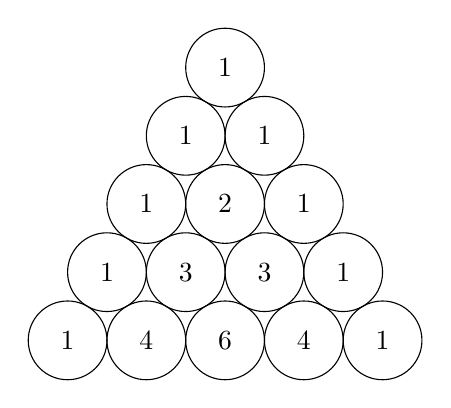
\begin{tikzpicture}[scale=1]
        \foreach \y in {0,...,4}{
          \foreach \x in {0,...,\y}
          {
            \pgfmathsetmacro{\nck}{int(\y!/(\x!*(\y-\x)!))}
            \draw ({\y/2-\x},{-\y*sqrt(3)/2}) circle (0.5) node {\nck};
          }
        }    
      \end{tikzpicture}    
\end{frame}
\subsection{History}
\begin{frame}
\frametitle{History}
\uncover<4->{Persian mathematician Omar Khaayyam(1048-1131) citing book by Al-Karaji(953-1029)}

\vspace{5mm}
\uncover<3->{}

\vspace{5mm}
\uncover<2->{Italian algebraist Nicolo Tartaglia in 1556}

\vspace{5mm}
French mathematician Blair Pascal in 1665.
\end{frame}
\section{Sierpinski Gasket}
\section{Dividing a circle into areas}
\end{document}